\section{Feature Description} %3.1

The extent of Arctic sea ice in the is deemed relevant to the following nine features. The content of carbon dioxide, the area of the ozone hole over the Arctic, the land and ocean temperature in the northern hemisphere, the Max/Ave/Min temperature of North Slope Alaska, the rainfall in the Arctic, daylight of Arctic and the population of the world.

\begin{figure}[htbp]
\center
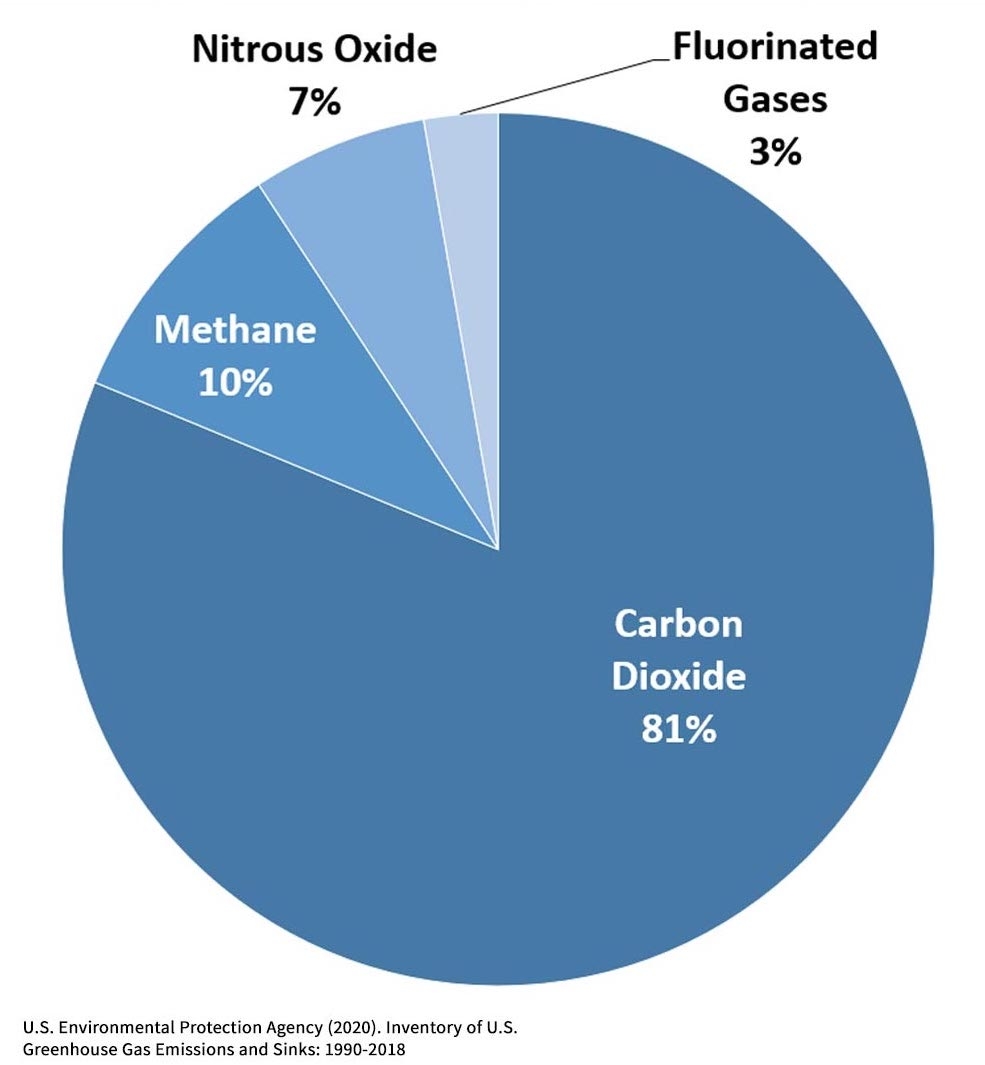
\includegraphics[width = 0.55\textwidth]{Figure/3.1-GreenHouseGas.jpg}
\longcaption{Overview of US Greenhouse Gases in 2018}{\label{3.1-GreenHouseGas} Overview of US Greenhouse Gases in 2018.\\ Image courtesy: https://www.epa.gov/ghgemissions/overview-greenhouse-gases}
\end{figure}

Changes in the area of sea ice in the Arctic are believed to be related to the content of carbon dioxide. As shown in Figure \ref{3.1-GreenHouseGas}, Carbon dioxide accounts for 81\% of greenhouse gases. Thus the main component of greenhouse gases is carbon dioxide, which is also the main cause of the greenhouse effect. According to J.H.Mercer, the greenhouse effect will have a catastrophic impact on the ice sheets \cite{mercer1978west}. Thus the content of carbon dioxide is chosen to be one of the features.

In addition, according to the results of the common correlated effects mean group (CCEMG) estimator, the GDP growth and the population size influence CO2 emission levels positively and significantly, at both the global and regional levels \cite{DONG2018180}. In that case, the GDP growth and the population size would have an impact on the ice sheets.

The ozone hole area is also considered to be related to the area of sea ice in the Arctic. In 2010, Sigmond and Fyfe found that the ozone depletion leads to a positive SAM response in austral summer, which induces sea ice melt \cite{sigmond2010has}. In that case, changes in the size of the ozone hole would also affect the changes in sea ice area. Thus the ozone hole area is chosen to be one of the features.

Furthermore, the temperature is deemed to be related to the area of sea ice in the Arctic. According to Ditlevsen and Grinsted's research, by considering a minimal model of an ice sheet, it shows that fluctuating temperatures have an effect on the mass balance and thus on the steady-state volume of the ice sheet \cite{mikkelsen2018influence}. Thus the temperature is considered to be a feature. In our project, we initially selected five different temperatures related to the Arctic area which are the ocean temperature in the Northern Hemisphere, the land temperature in the Northern Hemisphere, the maximum temperature of North Slope Alaska, the average temperature of North Slope Alaska, and the minimum temperature of North Slope Alaska.

Changes in the area of sea ice in the Arctic are also believed to be related to the rainfall. According to Bromwich and Robasky, the increased precipitation may reduce the net loss of ice sheets area or even turn it into net gain \cite{Bromwich1993RecentPT}. Thus rainfall is considered to be a feature.


The amount of daylight in the Arctic is also believed to be related to the area of ice sheets. The Arctic has polar day and polar night phenomena, so there is periodicity in the phenomenon of daylight. As shown in Figure \ref{3.1-daylight}, due to the sunshine could produce heat, thus different amount of daylight time would affect the temperature. Thus the daylight is considered to be a feature.


\begin{figure}[htbp]
\center
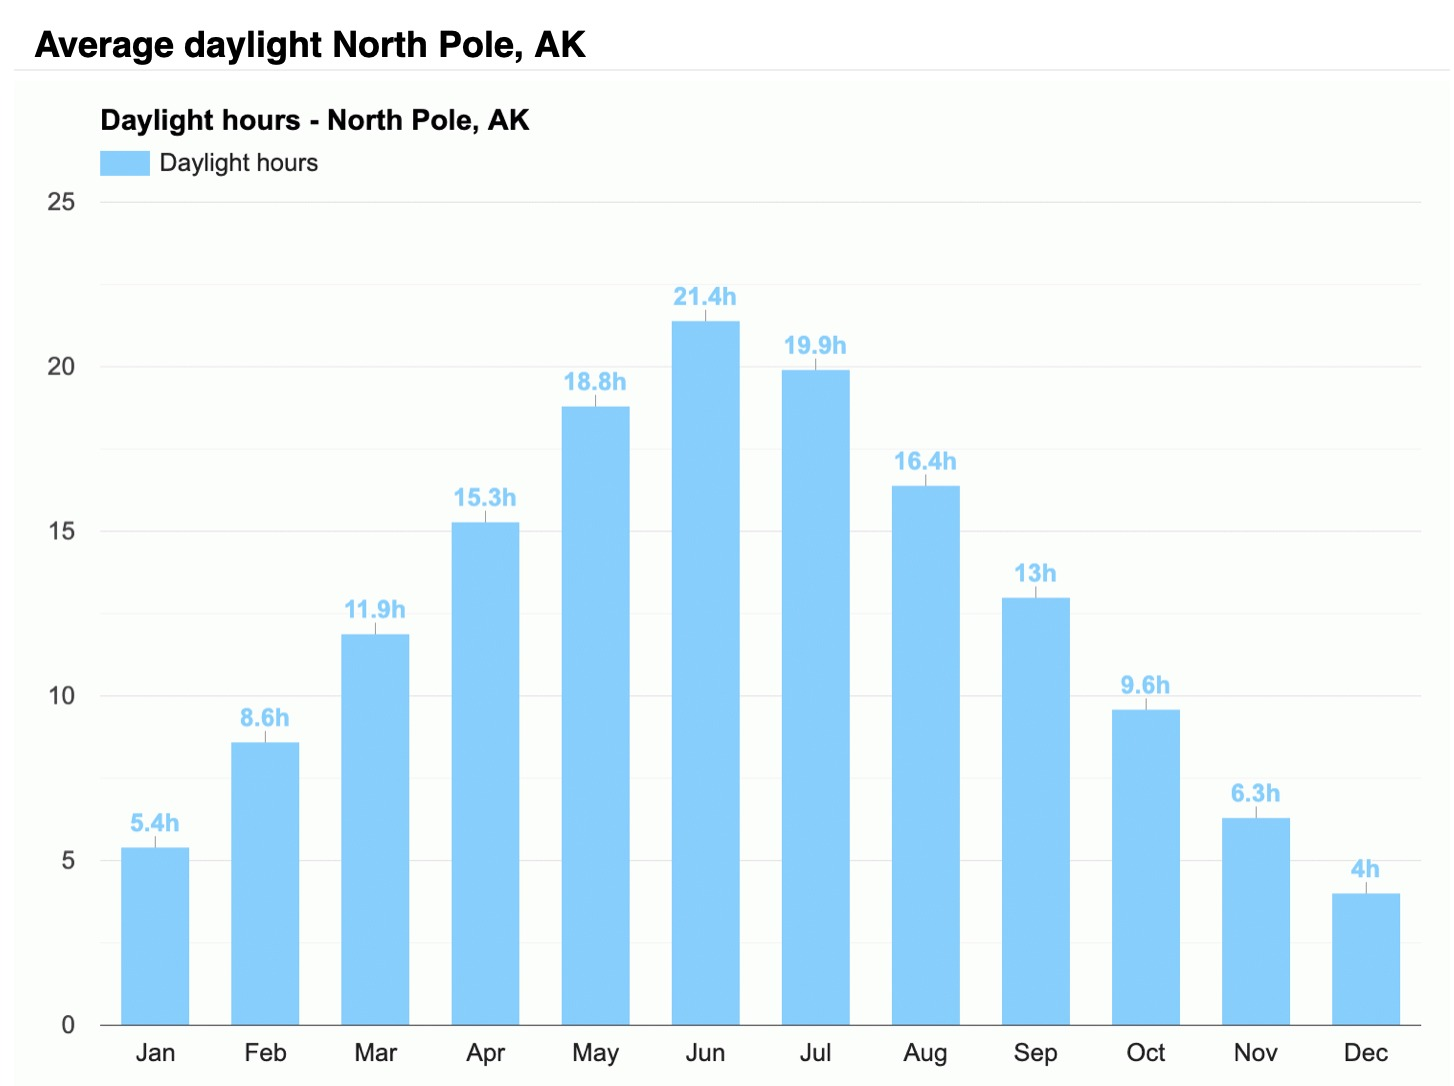
\includegraphics[width = 0.7\textwidth]{Figure/3.1-daylight.jpeg}
\longcaption{Average daylight in North Pole, Alaska}{\label{3.1-daylight} Average daylight in North Pole, Alaska. Image courtesy: https://www.weather-us.com/en/alaska-usa/north-pole-climate}
\end{figure}
